\chapter{Setting up the model}
Setting up your first model in GWTSA is relatively simple, and can be done with just a few lines of code. However, before we dive into the actual code to run a model and analyse the results, let us quickly go over the structure of modelling in GWTSA. There are basically three phases that the user has to go through, as visualized in the flow diagram shown in figure \ref{GWTSA_Flow}. 

\begin{figure}[h]
\label{GWTSA_Flow}
\centering
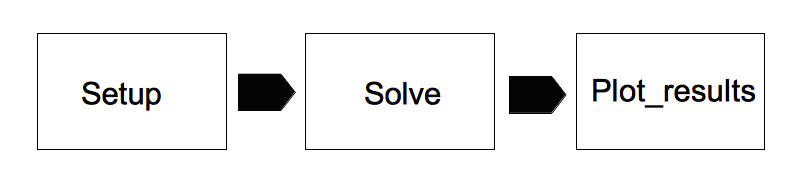
\includegraphics[width=1\linewidth]{Figures/GWTSA_Flow}
\caption{Flow diagram of the GWTSA modelling process}
\label{fig:GWTSA_Flow}
\end{figure}

In the first phase, an object is created for each borehole, and the necessary data is imported and prepared. This involved the determination of the time steps, model period etcetera. In the second phase, GWTSA performs the actual time series analysis and estimates the parameter values. It is in this phase that the model structure and important underlying assumptions can be chosen. The user is therefore encouraged to carefully read chapter 4 and choose the appropriate input arguments. The third phase is the analysis of th results, where GWTSA offers different graphs and numerics to interpret the model results.  

The first thing you want to do is open your python editor, and create a new .py file. The import of GWTSA can be done with the usual python import statements, if you have installed the software correctly. An example python file is available in the documentation folder to guide you through your first hands on experience. 

\section{Setup}
In this first phase the data necessary for a simulation is imported into an object. There are two important input files here: the observed groundwater levels and the climate data. Although the program is easy to adapt to your personal file format (simply change the np.loadtxt() input arguments), it is generally a good idea to use the input format similar to those in the Appendices of this manual. GWTSA will automatically select the right time steps, determine the model period and delete invalid observations from both time series. 

\textbf{Make sure to check the following:}
\begin{itemize}
\item{GWTSA expects a longer time series for the climate data than the groundwater data.}	
\item{The unit used throughout GWTSA is meters, so depending on the units of your input data, define by what value the data should be divided to get meters. Adapt input arguments `cl\_unit` and `gw\_unit` accordingly.}
\item{Set the right number of lines for both input files that GWTSA needs to skip when importing data using the 'rows' argument (groundwater and climate file respectively)}
\end{itemize}
	
\section{Solve}
Having set-up all the correct model data, a time series analysis can be performed by calling the 'solve' option. Here, there are two options that are important. The first is the model structure you want to use. Second, you need to provide a initial guess for the parameters, and here is where the hydrologists experience first enters the model. GWTSA can provide help on this, discussed in the next chapter 4. The software allows you to not provide a initial parameter estimate, but this is highly discouraged. The initial parameters need to be provided in a dictionary with parameter names that are similar as the model that is used. Although most of the parameter optimization is automatized, there are still many options available. To fully exploit these options read the advanced options section in chapter 4.

\textbf{Make sure to check the following:}
\begin{itemize}
	\item{Make sure the right parameters are provided in the dictionary}
	\item{Some of the parameters are scaled, take notice of this when providing the initial guess}
\end{itemize}

\section{Plot\_results}
Once we have estimated or optimized the parameters, we probably want to see what the resulting model looks like. We could run the simulate() function on our object, but the plot\_results function offers a neat way of simulating and viewing the resulting model. After running this function, the results window will pop up with a variety of information on your model. It combines different graphs of your data with the numerical values for some objective functions and the parameter values. This gives you the opportunity to visually check your model does what you expect it to do. 

\begin{figure}[h]
\centering
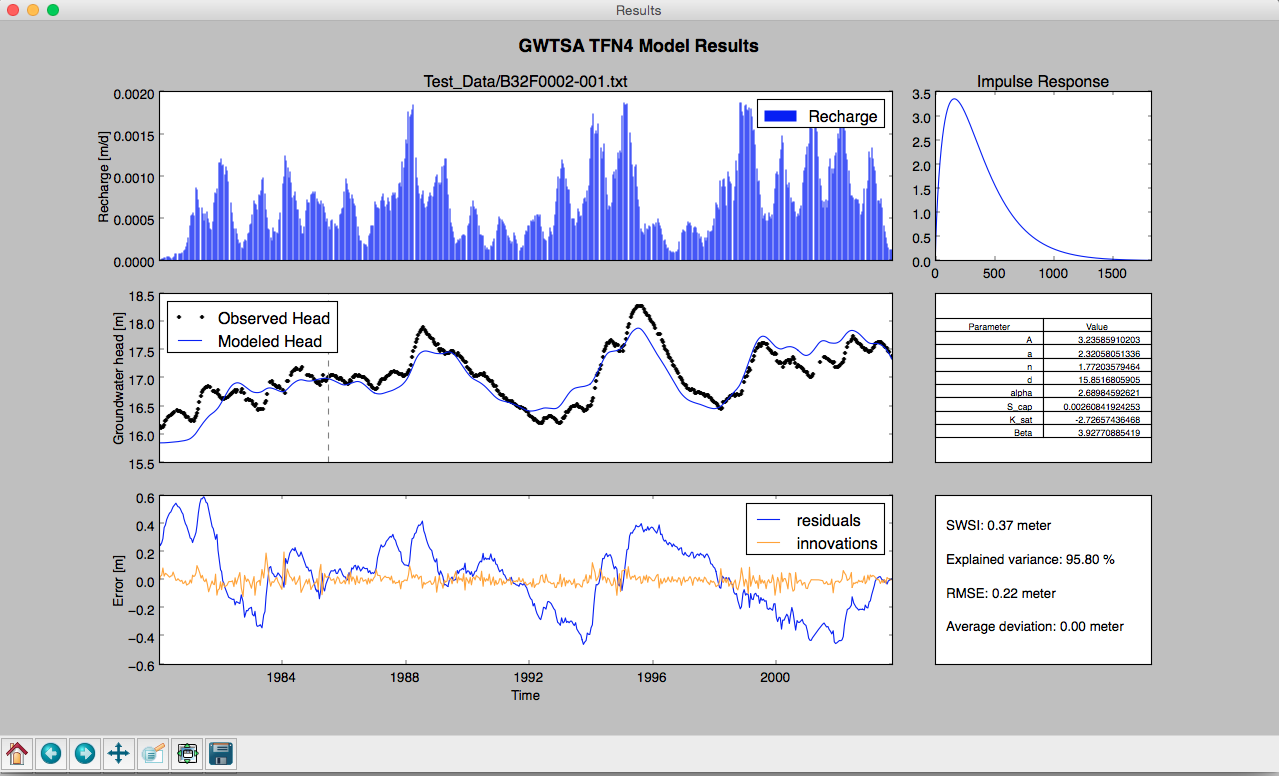
\includegraphics[width=1\linewidth]{Figures/plot_results}
\caption{Window showing the recharge, resulting model, model errors, impulse response shape and the parameter and objective function values}
\label{fig:plot_results}
\end{figure}


\section{Plot\_diagnostics}
It can sometimes be necessary to dive deeper into the parameter estimation process, to for example look at the evolution of the estimated parameter values or the correlation between parameters. Although it is always good to have a look at this window, it especially becomes useful when investigating new model structures. 

\begin{figure}[h]
\centering
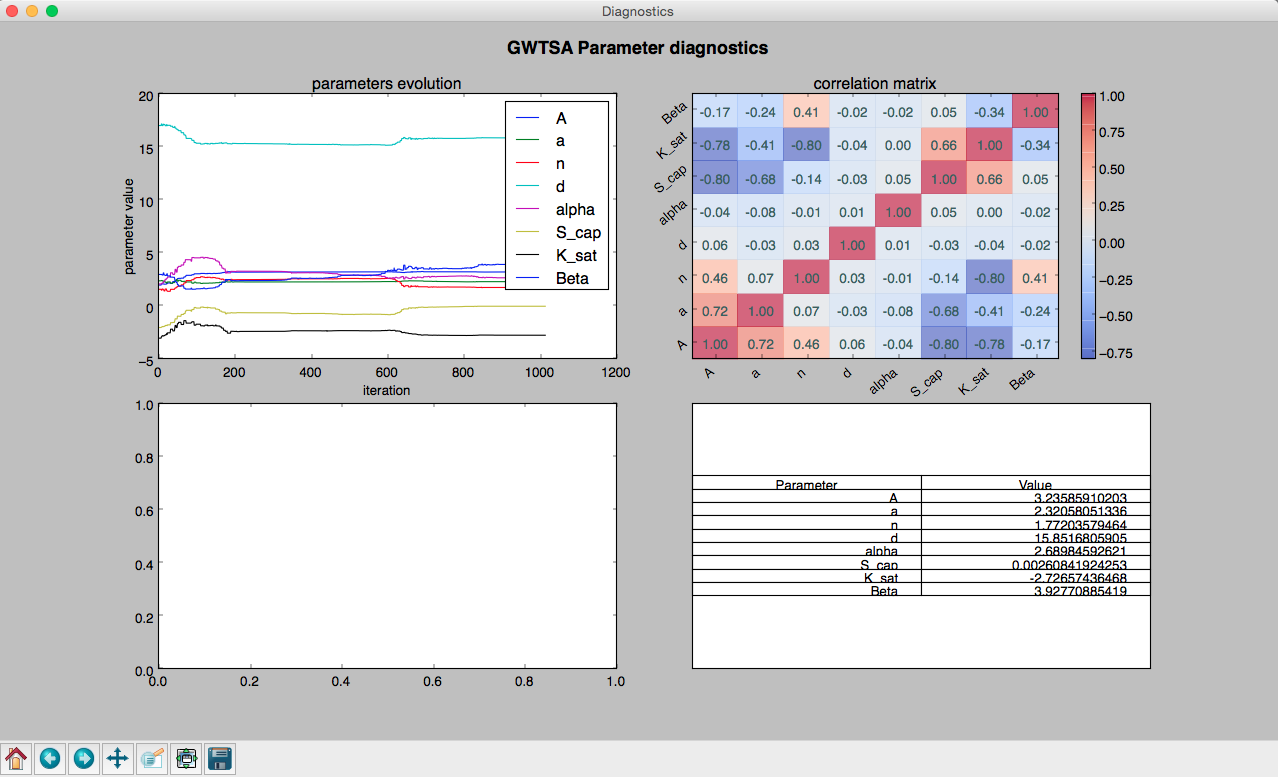
\includegraphics[width=1\linewidth]{Figures/plot_diagnostics}
\caption{Window showing the evolution of the parameters over the optimization, the correlation matrix and the final values for the parameters.}
\label{fig:plot_diagnostics}
\end{figure}

\section{Example script}
As stated in the introduction of this chapter, an entire simulation of GWTSA can be run with just a few lines of code. Below an example script to simulate the groundwater levels.

\begin{lstlisting}[language=Python]
from GWTSA import * 	# Import the entire GWTSA Toolbox

bore = 'Test_Data/GW_Levels.txt' #Groundwater Levels 
forcing = 'Test_Data/KNMI_Bilt.txt' # Climate Data
TFN = 'TFN4' # The Model structure

ts = Model(bore, forcing, rows=[5,8]) # Setup Phase

X0 = {'A': 3.0,'a': 2.2, 'n': 2.5,'Alpha': 10.0, 'S_cap': -1.00, 
		  'K_sat':-2.0, 'Beta': 3, 'D': -3, 'f': -0.1} 
		   # initial parameters as a dictionary

ts.solve(TFN, X0) # Solve Phase
ts.plot_results() # Results Phase
ts.plot_diagnostics() # Diagnostics Window
\end{lstlisting}
